\documentclass[t,11pt,aspectratio=169]{beamer}
\usepackage{tikz}
\usepackage{pgfplots}
\usetikzlibrary{calc}
\usepackage[utf8]{inputenc}
\usepackage[ngerman]{babel}
\usepackage{amsmath,amsfonts,amssymb}
\usepackage{framed}
\usecolortheme{orchid}
\usepackage{etoolbox}
\useinnertheme[shadow=true]{rounded}

\usepackage{verbatim}

%%% PROGRESSBAR
\definecolor{pbblue}{HTML}{D8D8D8}% filling color for the progress bar
\definecolor{pbgray}{HTML}{F2F2F2}% background color for the progress bar
\useoutertheme{infolines}
\setbeamerfont{footline}{size=\normalsize}
\setbeamersize{text margin left=30pt,text margin right=30pt}
\makeatletter
\setbeamertemplate{footline}
{
	\leavevmode%
	\hbox{%
		\begin{beamercolorbox}[wd=.333333\paperwidth,ht=2.5ex,dp=1ex,center]{title in head/foot}%
			\usebeamerfont{title in head/foot}\insertshorttitle
		\end{beamercolorbox}%
		\begin{beamercolorbox}[wd=.333333\paperwidth,ht=2.5ex,dp=1ex,center]{date in head/foot}%
			%\usebeamerfont{date in head/foot}\insertshortdate{}\hspace*{2em}
			%\insertframenumber\hspace*{2ex} 
		\end{beamercolorbox}
		\begin{beamercolorbox}[wd=.333333\paperwidth,ht=3ex,dp=1ex,center]{author in head/foot}%
			\usebeamerfont{author in head/foot}\insertshortauthor~~%\beamer@ifempty{\insertshortinstitute}{}{(\insertshortinstitute)}
		\end{beamercolorbox}%
	}%
	\vskip0pt%
}
\makeatother
\makeatletter
\def\progressbar@progressbar{} % the progress bar
\newcount\progressbar@tmpcounta% auxiliary counter
\newcount\progressbar@tmpcountb% auxiliary counter
\newdimen\progressbar@pbht %progressbar height
\newdimen\progressbar@pbwd %progressbar width
\newdimen\progressbar@tmpdim % auxiliary dimension
\progressbar@pbwd=\linewidth
\progressbar@pbht=1.5ex
\def\progressbar@progressbar{%
    \progressbar@tmpcounta=\insertpagenumber
    \progressbar@tmpcountb=\insertdocumentendpage
    \progressbar@tmpdim=\progressbar@pbwd
    \multiply\progressbar@tmpdim by \progressbar@tmpcounta
    \divide\progressbar@tmpdim by \progressbar@tmpcountb
  \begin{tikzpicture}[rounded corners=3pt,very thin]
    \shade[top color=pbgray!20,bottom color=pbgray!20,middle color=pbgray!50]
      (0pt, 0pt) rectangle ++ (\progressbar@pbwd, \progressbar@pbht);
      \shade[draw=pbblue,top color=pbblue!50,bottom color=pbblue!50,middle color=pbblue] %
        (0pt, 0pt) rectangle ++ (\progressbar@tmpdim, \progressbar@pbht);
    \draw[color=normal text.fg!50]  
      (0pt, 0pt) rectangle (\progressbar@pbwd, \progressbar@pbht) 
        node[pos=0.5,color=normal text.fg] {\textnormal{%
             \pgfmathparse{\insertpagenumber*100/\insertdocumentendpage}%
             \pgfmathprintnumber[fixed,precision=0]{\pgfmathresult}\,\%%
        }%
    };
  \end{tikzpicture}%
}
\addtobeamertemplate{headline}{}
{%
  \begin{beamercolorbox}[wd=\paperwidth,ht=4ex,center,dp=1ex]{white}%
    \progressbar@progressbar%
  \end{beamercolorbox}%
}
\makeatother

\setbeamertemplate{frametitle}[default][center]

%%% BLOCKS
% block = Aufgabe
\setbeamercolor{block title}{fg=black,bg=blue!30!white} 
\setbeamercolor{block body}{fg=black, bg=blue!3!white}

% alertblock = Definition
\setbeamercolor{block title alerted}{fg=black,bg=red!50!white} 
\setbeamercolor{block body alerted}{fg=black, bg=red!3!white}

% exampleblock = Wiederholung
\setbeamercolor{block title example}{fg=black,bg=green!30!white} 
\setbeamercolor{block body example}{fg=black, bg=green!3!white}

\setbeamercovered{transparent}
\setbeamertemplate{navigation symbols}{}

\addtocounter{page}{-1}
\addtocounter{framenumber}{-1}
\setbeamercovered{invisible}




\usepackage{fancyvrb}
\usepackage{xcolor}

\begin{document}
	
\begin{frame}{Was ist der Fehler 1. Art?}
Angenommen, wir testen statistisch die Hypothese $H_0$ gegen die Hypothese $H_1$.\\
Zum Beispiel: Ein Würfel ist fair ($H_0$) versus er ist gezinkt ($H_1$).
\pause
\vfill
\begin{center}
	\renewcommand{\arraystretch}{2.5}
	\begin{tabular}{c|c|c}
		& $H_0$ annehmen & $H_0$ verwerfen \\
		\hline
		$H_0$ ist wahr &  $\surd$  & Fehler 1. Art \\
		\hline
		$H_0$ ist falsch & Fehler 2. Art &  $\surd$ \\
	\end{tabular}
\end{center}
\vfill
\end{frame}

\begin{frame}
\begin{block}{Beispiel}
	Wir testen einen Würfel auf die Frage, ob er fair ist. Wir verwenden die Nullhypothese \glqq \textit{Der Würfel ist fair!}\grqq\ und die Gegenhypothese \glqq \textit{Der Würfel ist nicht fair!}\grqq. Bei unserem Test wird davon ausgegangen, dass der Würfel fair ist, wenn bei 50 Würfen mindestens 5 mal und höchstens 12 mal die 6 fällt. Wie groß ist die Wahrscheinlichkeit für den Fehler 1. Art?
\end{block}
\pause
\begin{itemize}
	\item $H_0:$ Würfel ist fair, $H_1:$ Würfel ist nicht fair
	\item Stichprobenumfang $n=50$, Testgröße $X=$ Anzahl der 6en
	\item Annahmebereich $\{ 5,...,12 \}$
	\item Ablehnungsbereich $\{ 0,...,4,13,...,50 \}$
\end{itemize}
\end{frame}

\begin{frame}{Wie ist $X$ unter $H_0$ verteilt?}
\begin{itemize}
\item Binomialverteilung
\item $n=50$
\item $p=\frac{1}{6}$
\end{itemize}
\pause
\vfill
\begin{center}
	\usebeamerfont{frametitle}\usebeamercolor[fg]{frametitle} Wann begehen wir den Fehler 1. Art?
\end{center}
\vfill
\begin{itemize}
\item $H_0$ verwerfen obwohl $H_0$ wahr ist
\item die Anzahl der 6en liegt nicht im Annahmebereich, obwohl der Würfel fair ist
\item $X\notin \{ 5,...,12 \}$, $X\sim \mathcal{B}(n=50,p=1/6)$
\end{itemize}
\end{frame}

\begin{frame}{Wie hoch ist die Wahrscheinlichkeit für den Fehler 1. Art?}
\begin{itemize}[<+->]
\item $X\notin \{ 5,...,12 \}$, $X\sim \mathcal{B}(n=50,p=1/6)$
\item $\mathbf{P}(X\notin \{ 5,...,12 \})$
\item[] $= \mathbf{P}(X\leq 4) + \mathbf{P}(X\geq  13)$
\item[] $= \mathbf{P}(X\leq 4) + 1- \mathbf{P}(X\leq  12)$
\item[] $=$ \texttt{pbinom(4,50,1/6)} + 1 - \texttt{pbinom(12,50,1/6)}
\item[] $= 0.0643 + 1 - 0.9373 =  0.1270 $
\end{itemize}
\end{frame}

\begin{frame}[fragile]{Wie können wir den Fehler 1. Art beschränken?}
\begin{minipage}[t]{0.5\textwidth}
	\begin{Verbatim}[fontsize=\small, commandchars=\\\{\}]
	> x <- 0:50
	> f <- dbinom(x,50,1/6)
	> plot(x,f,type="h")
	
	> reject <- \textcolor{red}{c(0:4,13:50)}
	> f_reject <- dbinom(reject,50,1/6)
	> lines(reject,f_reject,col="red",type="h")
	> mtext(round(sum(f_reject),4),side=3,col="red")
	\end{Verbatim}
\end{minipage}
\hfill
\begin{minipage}{0.4\textwidth}
	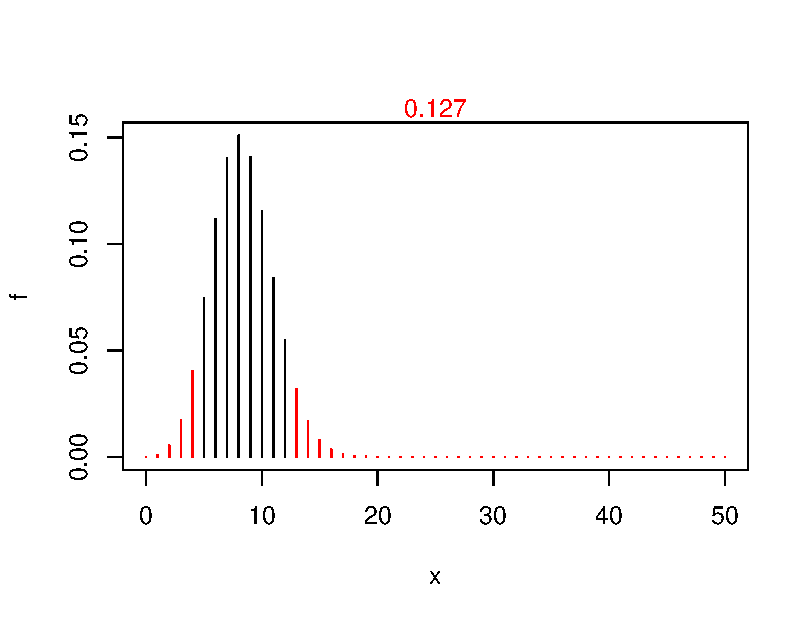
\includegraphics[width=\textwidth]{Rplot02.pdf}
\end{minipage}
\end{frame}

\begin{frame}[fragile]{Wie können wir den Fehler 1. Art beschränken?}
\begin{minipage}[t]{0.5\textwidth}
	\begin{Verbatim}[fontsize=\small, commandchars=\\\{\}]
	> x <- 0:50
	> f <- dbinom(x,50,1/6)
	> plot(x,f,type="h")
	
	> reject <- \textcolor{red}{c(0:3,14:50)}
	> f_reject <- dbinom(reject,50,1/6)
	> lines(reject,f_reject,col="red",type="h")
	> mtext(round(sum(f_reject),4),side=3,col="red")
	\end{Verbatim}
\end{minipage}
\hfill
\begin{minipage}{0.4\textwidth}
	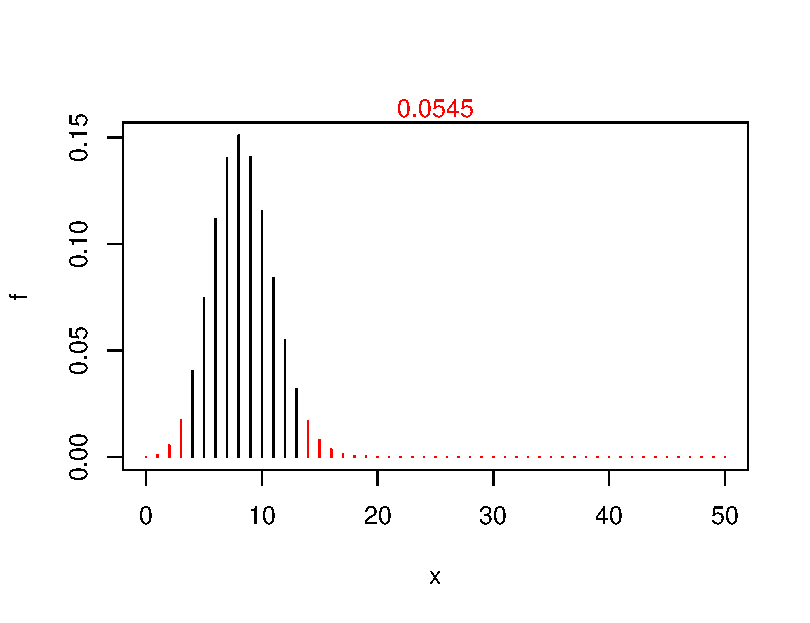
\includegraphics[width=\textwidth]{Rplot03.pdf}
\end{minipage}
\end{frame}

\end{document}